\section{Stage 5: Basic HTML5 game development: the game loop}

\begin{frame}[fragile]
  \begin{center}
    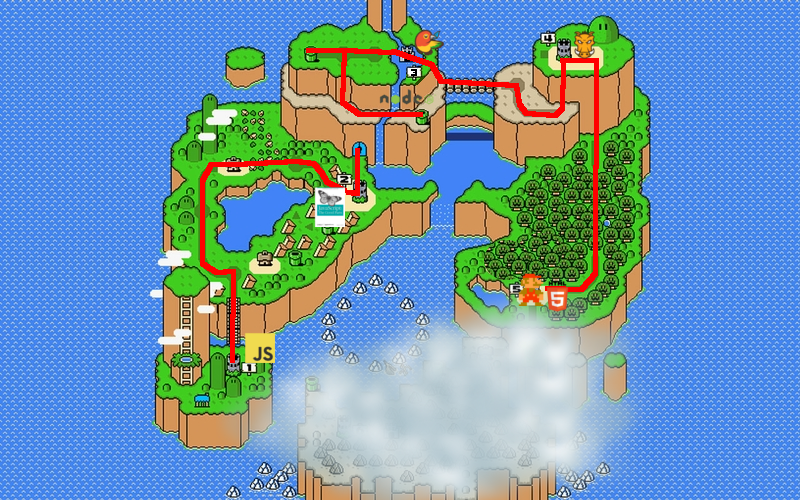
\includegraphics[width=300px]{images/map_stage_5.png}
  \end{center}
\end{frame}

\begin{frame}[fragile]
  \frametitle{Game design}

  We are going to create a simple game in the following stages using Javascript. The game will be a tiny MOBA (Multiplayer Online Battle Arena) and it will have the following features:

  \pause

  \begin{itemize}
    \pause \item Player choose a team: red or blue
    \pause \item Player choose between 3 classes:
      \begin{itemize}
        \item Soldier: low hp, ranged weapon, medium damage
        \item Knight: medium hp, melee weapon, high damage
        \item Protector: high hp, no weapon, can block enemy's attacks
      \end{itemize}
    \pause \item \textbf{Objective:} Destroy other's team base
  \end{itemize}
\end{frame}

\begin{frame}[fragile]
  \frametitle{Game loop}

  \ldots
\end{frame}

\begin{frame}[fragile]
  \frametitle{HTML5}

  First of all, HTML5 is not a programming language, neither an API. It's the 5th revision of HTML but also an umbrella term about 100 specifications for the next generation web applications.
  Visit \url{http://platform.html5.org/} to have a global view about it.

  \pause

  We are going to use a small subset of these new APIs:
  \begin{itemize}
    \pause \item \textbf{Canvas:} Drawing graphics in 2D.
    \pause \item \textbf{requestAnimationFrame:} Handling animations timings.
    \pause \item \textbf{Websockets:} Two-way communication between browser and server.
  \end{itemize}
\end{frame}

\begin{frame}[fragile]
  \frametitle{Introduction to the Canvas API}

  HTML5 introduces a new tag called \texttt{canvas}. Using Javascript we can interact with this element in order to draw 2D graphics in real time.

  \begin{block}{Canvas element and 2d context}
  {\scriptsize
  \begin{verbatim}
  <canvas id=``gameArea'' width=``200'' height=``200''></canvas>
  <script>
  var canvas = document.getElementById('gameArea'),
      ctx = canvas.getContext(``2d'');
  </script>
  \end{verbatim}
  }
  \end{block}
\end{frame}

\begin{frame}[fragile]
  \frametitle{Introduction to the Canvas API}

  \begin{block}{Drawing lines}
  {\scriptsize
  \begin{verbatim}
  ctx.fillStyle = ``black'';

  ctx.beginPath();
  ctx.moveTo(10, 10);
  ctx.lineTo(100, 10);
  ctx.stroke();

  ctx.beginPath();
  ctx.moveTo(10, 20);
  ctx.lineTo(100, 20);
  ctx.stroke();

  ctx.beginPath();
  ctx.moveTo(10, 30);
  ctx.lineTo(100, 30);
  ctx.stroke();
  \end{verbatim}
  }
  \end{block}
\end{frame}

\begin{frame}[fragile]
  \frametitle{Introduction to the Canvas API}

  \begin{block}{Drawing rects}
  {\scriptsize
  \begin{verbatim}
  ctx.fillStyle = ``blue'';
  ctx.strokeStyle = ``red'';
  ctx.fillRect(100, 100, 50, 50);
  ctx.strokeRect(165, 165, 25, 25);
  \end{verbatim}
  }
  \end{block}

  \pause

  \begin{block}{Drawing arcs}
  {\scriptsize
  \begin{verbatim}
  ctx.beginPath();
  ctx.fillStyle = ``green'';
  ctx.strokeStyle = ``orange'';
  ctx.arc(150, 50, 5, 0, 2 * Math.PI);
  \end{verbatim}
  }
  \end{block}
\end{frame}

\begin{frame}[fragile]
  \frametitle{Introduction to the Canvas API}

  \begin{block}{Drawing images}
  {\scriptsize
  \begin{verbatim}
  var crate = new Image();
  crate.src = 'images/crate.png';
  /*
  * onload callback function. Called when the
  * image is ready to be drawn.
  */
  crate.onload = function () {
      ctx.drawImage(crate, 100, 100);
  };
  \end{verbatim}
  }
  \end{block}
\end{frame}

\begin{frame}[fragile]
  \frametitle{Introduction to the Canvas API}

  \begin{block}{\texttt{scale}}
  {\tiny
  \begin{verbatim}
  // Draw crate 2x bigger
  ctx.scale(2, 2);
  ctx.drawImage(crate, 100, 100);
  \end{verbatim}
  }
  \end{block}

  \pause

  \begin{block}{\texttt{translate}}
  {\tiny
  \begin{verbatim}
  // Same as ctx.drawImage(create, 100, 100);
  ctx.translate(100, 100);
  ctx.drawImage(crate, 0, 0);
  \end{verbatim}
  }
  \end{block}

  \pause

  \begin{block}{\texttt{rotate}}
  {\tiny
  \begin{verbatim}
  ctx.rotate(45 * (Math.PI * 180));
  ctx.drawImage(crate, 0, 0);
  \end{verbatim}
  }
  \end{block}
\end{frame}

\begin{frame}[fragile]
  \frametitle{Introduction to the Canvas API}

  \begin{block}{\texttt{save} and \texttt{restore}}
  {\tiny
  \begin{verbatim}
  ctx.save();
  ctx.translate(100, 100);
  ctx.translate(crate.width / 2, crate.height / 2);
  ctx.rotate(45 * (Math.PI / 180));
  ctx.translate(-crate.width / 2, -crate.height / 2);
  ctx.drawImage(crate, 0, 0);
  ctx.restore();

  ctx.drawImage(create, 0, 0);
  \end{verbatim}
  }
  \end{block}
\end{frame}

\begin{frame}[fragile]
  \frametitle{\texttt{requestAnimationFrame}}

  Our game must run on 60 fps (frames per second) in order to be smoothly. It means, we must execute the game loop 60 times each second or 1 time each 1000 / 60 milliseconds.

  \pause

  \begin{block}{Using \texttt{setInterval}}
  {\scriptsize
  \begin{verbatim}
    setInterval(function () {
        console.log(``Game loop!'');
    }, 1000 / 60);
  \end{verbatim}
  }
  \end{block}

  \pause

  \begin{block}{Using \texttt{requestAnimationFrame}}
  {\scriptsize
  \begin{verbatim}
    function gameLoop() {
      requestAnimationFrame(gameLoop);
      console.log(``Game loop!'');
    }

    gameLoop();
  \end{verbatim}
  }
  \end{block}
\end{frame}
